%-----------------------------------------------------------------
%	LÍNIES ESPECTRALS
%	!TEX root = ./../main.tex
%-----------------------------------------------------------------
\section{Línies espectrals}
\subsection{Història}
\begin{itemize}
	\item  William Wollaston (1802) descobreix que la llum solar a través d'un prisma produeix un espectre tipus arc iris amb ratlles fosques superimposades (a l'espectre continu) a les longituds d'ona a les quals la llum solar havia estat absorbida (i.e., ratlles, o línies, d'absorció).
	\item  Joseph Fraunhofer (1814) va catalogar 475 d'aquestes ratlles d'absorció, les quals van resultar coincidir amb les produïdes per sals en una flama.
	\item Bunsen \& Kirchhoff van inventar l'espectroscopi. Aquest fa passar la llum d'una flama a través d'un prisma per ser analitzada. Kirchhoff va determinar 70 línies fosques en l'espectre solar corresponent a 70 línies brillants emeses (al laboratori) per vapor de ferro.

	Així doncs, els elements químics poden ser identificats sense ambigüitat per les seves línies espectrals, com si es tractessin d'empremtes dactilars.
\end{itemize}

%-----------------------------------------------------------------
\subsection{Lleis de Kirchhoff}
\begin{enumerate}[(i)]
	\item Un gas dens i calent (o un sòlid calent) produeix un espectre de radiació continu sense línies fosques.
	\item Un gas calent i difús produeix línies brillants (línies d'emissió).
	\item Si la llum d'una font d'espectre continu travessa un gas fres i difús, ratlles espectrals fosques (línies d'absorció) se superposen sobre l'espectre continu.
\end{enumerate}
D'aquesta manera es va poder identificar un gran nombre d'elements químics al Sol i a les estrelles, tot advertint-se que a diferents estrelles els correspon diferent espectre (ja que la composició química varia d'una estrella a una altra).
\begin{figure}[H]
	\centering
	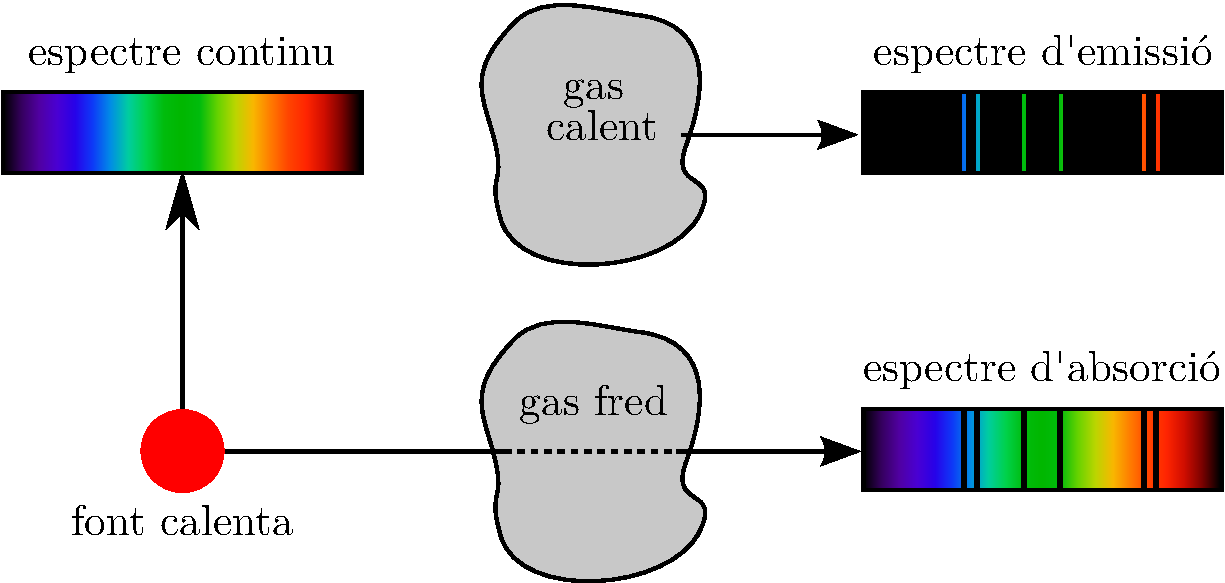
\includegraphics[width=0.75\textwidth]{./images/3-kirchhoff}
	\caption{Representació dels diferents espectres regits per les lleis de Kirchhoff}
	\label{fig:kirchhoff}
\end{figure}

\subsubsection*{Model de Bohr}
Les línies d'emissió són degudes al fotó emès en saltar un electró d'un nivell de major energia a un de menor energia. El procés oposat dóna lloc a línies d'absorció.
\begin{figure}[h]
	\centering
	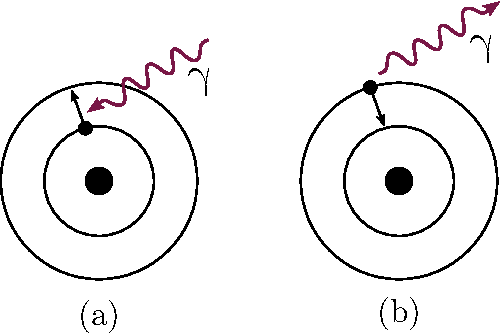
\includegraphics[width=0.4\textwidth]{./images/3-photon-abs-em}
	\caption{Absorció d'un fotó (a), i emissió d'un fotó (b)}
	\label{fig:photon-abs-em}
\end{figure}

En el model atòmic de Bohr
\begin{align}
	E_{n} = -\frac{13.6}{n^{2}} \si{\eV} \Rightarrow E_{\gamma} = E_{b} - E_{a} = 13.6 \qty(\frac{1}{n_{a}^{2}} - \frac{1}{n_{b}^{2}}) > 0
\end{align}
on $n$ és el nombre quàntic principal i $n_{a} < n_{b}$.
\begin{figure}[ht]
	\centering
	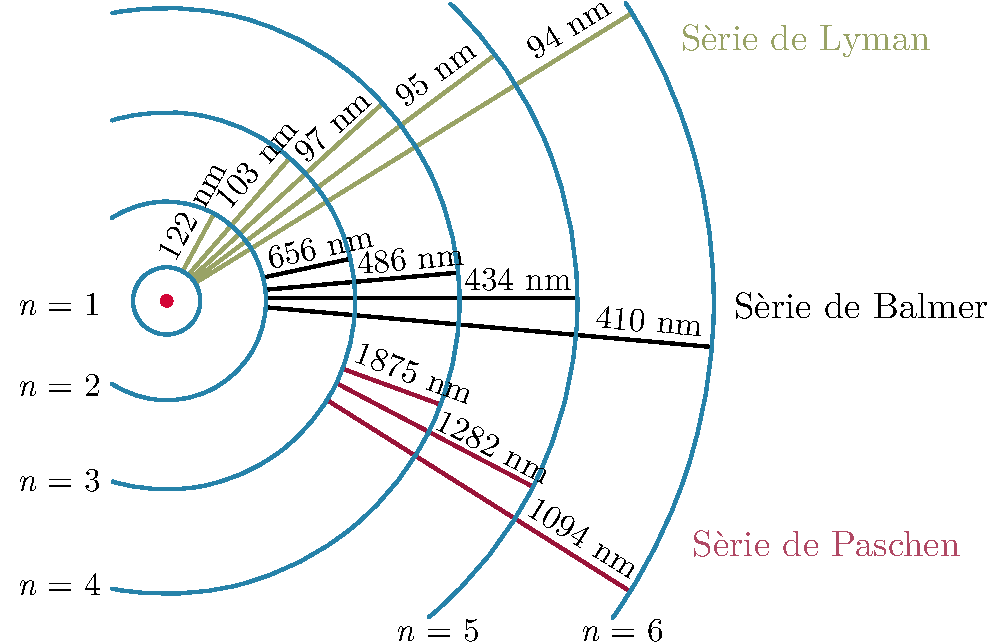
\includegraphics[width=0.7\textwidth]{./images/3-hydrogen-transitions}
	\caption{Transicions electròniques i les seves longituds d'ona resultants en l'emissió per a l'àtom d'hidrogen}
	\label{fig:hydrogen-transitions}
\end{figure}

\subsubsection*{Efecte Zeeman}
Divisió de les línies espectrals per la presència d'un camp magnètic d'intensitat $B$. En particular es compleix
\begin{align}
	\nu = \nu_{0} \pm \frac{eB}{4\pi \mu c}
\end{align}
on $e$ és la càrrega de l'electró, i $\mu$ és la massa reduïda.
\begin{figure}[h]
	\centering
	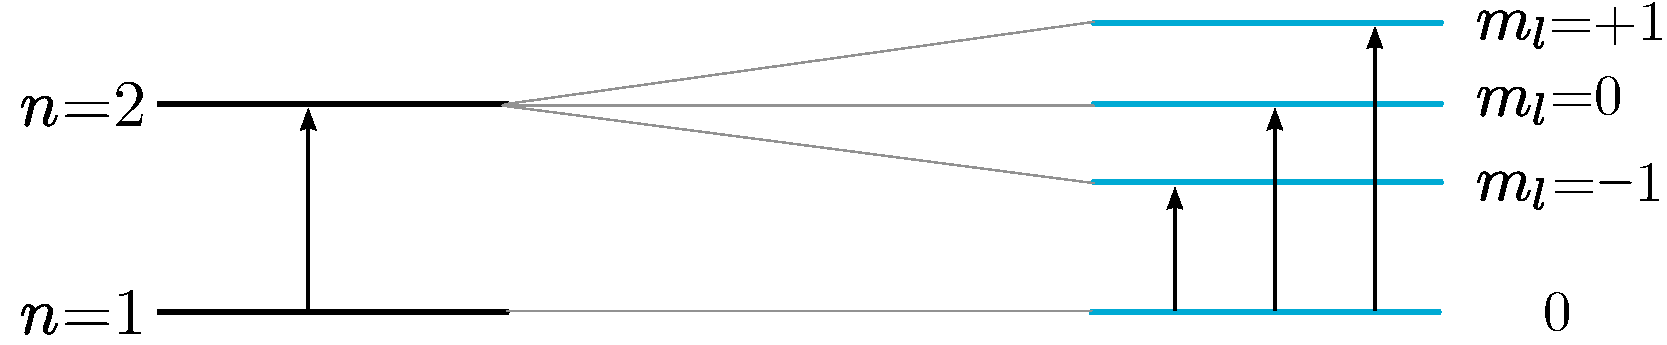
\includegraphics[width=0.7\textwidth]{./images/3-zeeman}
	\caption{Divisió de les línies d'absorció per efecte Zeeman}
	\label{fig:zeeman}
\end{figure}

La divisió de les línies espectrals indica la presència de camps magnètics, tal com passa a les taques solars.

%-----------------------------------------------------------------
\subsection{Seqüència dels espectres estel·lars de Harvard}
% FIXME: cannon@sec:bio
La catalogació que Annie Jump Cannon (1863), astrònoma americana, va fer de les estrelles ha estat fonamental per l'actual classificació estel·lar. La classificació espectral de Harvard va en sentit decreixent de temperatures: O B A F G K M R N S. Cada lletra, alhora, se subdivideix en deu (e.g., A0-A9).

Per facilitat, s'acostuma a fer servir la següent regla mnemotècnica per recordar els tipus d'espectres estel·lars:
\begin{quote}
	\textit{‘Oh! Be A Fine Girl, Kiss Me Right Now, Sweetheart!’}
\end{quote}

A continuació podeu consultar una taula que resumeix la classificació espectral estel·lar de Harvard.
\begin{table}[H]
	\centering
		\begin{tabular}{ccccc}
		\toprule
		Tipus & $M$ ($\times \si{\Msun}$) & $R$ ($\times \si{\Rsun}$) & $L$ ($\times \si{\Lsun}$) & $T$ ($\times \SI{e3}{\K}$) \\
		\midrule
		O & \numrange{20}{100} & $\sim\num{15}$ & \numrange{e5}{e6} & \numrange{30}{50} \\
		B & \numrange{3}{18} & $\sim\num{7}$ & \numrange{100}{52000} & \numrange{10.5}{30} \\
		A & \numrange{1.5}{3} & $\sim\num{2.5}$ & \numrange{7}{50} & \numrange{7.2}{9.5} \\
		F & \numrange{1.2}{1.6} & $\sim\num{1.3}$ & \numrange{2}{6.5} & \numrange{6.1}{7.2} \\
		G & \numrange{0.8}{1.1} & $\sim\num{1.1}$ & \numrange{0.4}{2} & \numrange{5.3}{6} \\
		K & \numrange{0.5}{0.8} & $\sim\num{0.9}$ & \numrange{0.1}{0.4} & \numrange{3.9}{5.2} \\
		M & $< \num{0.5}$ & $\sim\num{0.4}$ & $<\num{0.08}$ & $<\num{3.9}$ \\
		\bottomrule
		\end{tabular}
	\caption{Comparació de les característiques físiques de les estrelles de la seqüència principal}
	\label{tab:harvard}
\end{table}

\begin{figure}[h]
	\centering
	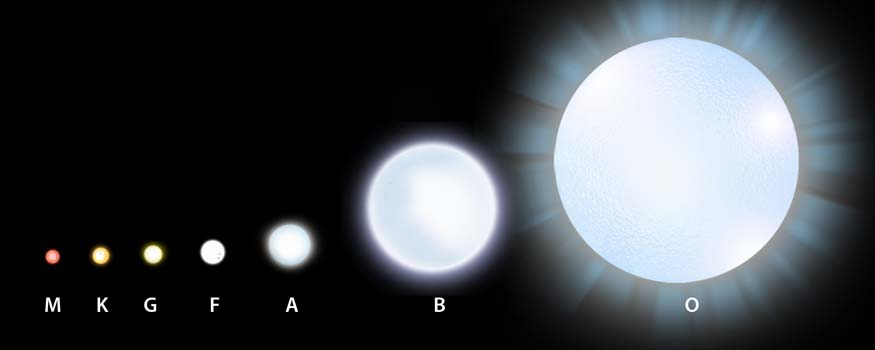
\includegraphics[width=0.8\textwidth]{./images/3-harvard-classification}
	\caption{Comparació visual dels diferents tipus d'espectres estel·lars de la classificació de Harvard}
	\label{fig:harvard-classification}
\end{figure}

%-------------------------------
\subsubsection*{Estrelles tipus O}
Les més brillants, calents i massives de la seqüència principal. De color blau, emeten la major part de la seva energia en l'ultraviolat.

Posseeixen una temperatura efectiva entre $\SI{30 e3}{\K}$ i valors superiors a $\SI{50 e3}{\K}$ i una lluminositat entre $\SI{e5}{\Lsun}$ i valors més enllà de $\SI{e6}{\Lsun}$. Les seves masses varien entre $\SI{20}{\Msun}$ i $\SI{100}{\Msun}$. Cremen combustible nuclear a un ritme molt elevat, de forma que només \textit{viuen} de 3 a 6 milions d'anys.

Com a conseqüència de la seva alta temperatura, les línies de l'hidrogen dels seus espectres són febles. Les línies que dominen són les de He II.

Són escasses, només es coneixen un grapat del tipus O3 i O4 (no es coneix cap estrella de O0 a O2).

Les més brillants a simple vista són Delta Orionis i Zeta Orionis (ambdues O9 supergegants).

%-------------------------------
\subsubsection*{Estrelles tipus B}
Els seus espectres són dominats per les línies d'absorció de l'hidrogen i de l'heli neutre. Són de color blau i calents. Emeten principalment en l'ultraviolat.

En la seqüència principal les seves temperatures se situen en l'interval de $\SI{10500}{\K}$ a $\SI{30000}{\K}$, amb lluminositats de $\SI{100}{\Lsun}$ a $\SI{52000}{\Lsun}$ i masses de $\SI{3}{\Msun}$ a $\SI{18}{\Msun}$.

Les supergegants posseeixen masses de fins a $\SI{25}{\Msun}$ i lluminositats de fins a $\SI{260 e3}{\Lsun}$. Rigel és una supergegant, mentre que Spica [\href{http://apod.nasa.gov/apod/ap021214.html}{APOD~021204}] i Regulus són estrelles nanes.

Viuen només unes desenes de milions d'anys.

%-------------------------------
\subsubsection*{Estrelles tipus A}
Els seus espectres són dominats per les línies d'absorció de l'hidrogen. En aquests espectres es donen les línies d'absorció més intenses en estrelles de la seqüència principal. Són de color blau-blanquinós.

Les de la seqüència principal posseeixen temperatures en el rang de $\SI{7200}{\K}$ a $\SI{9500}{\K}$ i són entre 7 i 50 vegades més lluminoses que el Sol, amb masses entre 1.5 i 3 masses solars.

Les supergegants (com Deneb [\href{http://apod.nasa.gov/apod/ap961212.html}{APOD~961212}]) són més massives (fins a $\SI{16}{\Msun}$), amb temperatures de fins a $\SI{9700}{\K}$ i lluminositats per sobre de $\SI{35000}{\Lsun}$.

Sírius és de tipus espectral A1 i Vega és del tipus A0.

%-------------------------------
\subsubsection*{Estrelles tipus F}
Les línies d'absorció de l'hidrogen decauen fortament en intensitat del tipus F0 al F9 al temps que les línies del calci augmenten en intensitat i moltes altres línies corresponents a metalls comencen a fer-se visibles.

Les de la seqüència principal posseeixen temperatures entre $\SI{6100}{\K}$ i $\SI{7200}{\K}$, mentre que les supergegants són uns pocs centenars de kelvin més fredes.

Les masses en la seqüència principal se situen entre $\SI{1.2}{\Msun}$ i $\SI{1.6}{\Msun}$; les lluminositats, entre $\SI{2}{\Lsun}$ i $\SI{6.5}{\Lsun}$. Les supergegants tenen fins a 12 vegades la massa del Sol i lluminositats de fins a $\SI{32000}{\Lsun}$.

Les estrelles Polaris [\href{http://apod.nasa.gov/apod/ap991006.html}{APOD~991006}] i Procyon són de tipus F.

%-------------------------------
\subsubsection*{Estrelles tipus G}
Les pertanyents a la seqüència principal tenen temperatures efectives entre $\SI{5300}{\K}$ i $\SI{6000}{\K}$, per això són de color groc. Les gegants són entre 100 i 500 kelvin més fredes i les supergegants posseeixen temperatures entre $\SI{4500}{\K}$ i $\SI{5500}{\K}$.

L'espectre del Sol (tipus G2) és dominat per línies de l'ió \ch{Ca+} i de metalls neutres. En estrelles de tipus G més fredes comencen a advertir-se les bandes de \ch{CH} i \ch{CN}.

Les masses en la seqüència principal i de les gegants varien entre $\SI{0.8}{\Msun}$ i $\SI{1.1}{\Msun}$; la massa de les supergegants varia entre $\SI{10}{\Msun}$ i $\SI{12}{\Msun}$.

Les lluminositats de les gegants varia entre $\SI{30}{\Lsun}$ i $\SI{60}{\Lsun}$; les lluminositats de les supergegants, entre $\SI{10000}{\Lsun}$ i $\SI{300000}{\Lsun}$.

L'estrella Capella\footnote{[\href{http://apod.nasa.gov/apod/ap021106.html}{APOD~021106}]: l'Hexàgon Hivernal és format per Aldebaran, Capella, Castor, Procyon, Rigel, i Sírius.} és una gegant de tipus G.

%-------------------------------
\subsubsection*{Estrelles tipus K}
En la seqüència principal tenen temperatures entre $\SI{3900}{\K}$ i $\SI{5200}{\K}$, les gegants són entre 100 i 400 kelvin més fredes i les supergegants són uns quants centenars de kelvin més fredes encara. Són de color taronja.

Les masses en la seqüència principal van entre $\SI{0.5}{\Msun}$ i $\SI{0.8}{\Msun}$; les seves lluminositats, entre $0\SI{0.1}{\Lsun}$ i $\SI{0.4}{\Lsun}$. Les gegants posseeixen masses entre $\SI{1.1}{\Msun}$ i $\SI{1.2}{\Msun}$ i lluminositats entre $\SI{60}{\Lsun}$ i $\SI{300}{\Lsun}$. Les supergegants, com a màxim, arriben a $\SI{13}{\Msun}$ i $\SI{40000}{\Lsun}$.

Els seus espectres es caracteritzen per línies d'absorció del ferro i titani neutres, i calci neutre i \ch{Ca+} (aquestes dues últimes són línies intenses). La intensitat de les bandes de \ch{CN} i \ch{TiO} es reforcen notablement des de K0 fins a K9.

Arcturus [\href{http://apod.nasa.gov/apod/ap020910.html}{APOD~020910}] és una gegant K1 i Aldebaran és una gegant K5.

%-------------------------------
\subsubsection*{Estrelles tipus M}
Són estrelles de molt baixa temperatura efectiva (inferior a $\SI{3900}{\K}$) de color vermellós. Emeten la major part de la seva radiació en l'infraroig.

Les nanes tipus M (conegudes com \textit{nanes rojes}) se situen al tram inferior de la seqüència principal. Com que posseeixen lluminositats de $\SI{0.08}{\Lsun}$ com a màxim, ni tan sols les més properes a nosaltres (e.g., Proxima Centauri) poden ser vistes sense telescopi. Les seves masses, en la seqüència principal, no arriben a $\SI{0.5}{\Msun}$.

La seva vida mitjana podria ser major que l'edat actual de l'Univers.

Moltes estrelles tipus M són gegants amb masses entre $\SI{1.2}{\Msun}$ i $\SI{1.3}{\Msun}$ i amb lluminositats en torn a $\SI{300}{\Lsun}$.

Les supergegants, com Betelgeuse i Antares, posseeixen masses entre $\SI{13}{\Msun}$ i $\SI{25}{\Msun}$ i lluminositats entre $\SI{40000}{\Lsun}$ i $\SI{500000}{\Lsun}$. La seva mida pot ser tan gran com l'òrbita de Júpiter.

Els seus espectres solen ser dominats per amples bandes d'absorció moleculars, com el \ch{TiO}, però també són presents línies d'absorció de metalls neutres.

%-------------------------------
\subsubsection*{Estrelles tipus R \& N (\textsl{carbon stars})}
Gegants roges i fredes en avançat estat d'evolució. Els seus espectres són dominats per fortes bandes corresponents a les molècules \ch{CN}, \ch{CH}, i \ch{C2} (per això el nom de \textit{carbon stars}).

La presència de \ch{Li} indica que aquests elements (\ch{C}, \ch{Li}, \ch{N}) han estat produïts al nucli de l'estrella mitjançant reaccions nuclears i transportats per convecció a la superfície.

Ja que el carbó només es pot produir pel procés triple--$\alpha$ a molt alta temperatura, aquestes estrelles es troben en un estat evolutiu força avançat.

Les estrelles tipus R posseeixen temperatura efectiva entre $\SI{4000}{\K}$ i $\SI{5000}{\K}$; les tipus N, aproximadament $\SI{3000}{\K}$.

Les tipus R poden ser fins a 10 vegades més lluminoses que les tipus N.

%-------------------------------
\subsubsection*{Estrelles tipus S}
Gegants roges d'espectre similar a les del tipus $M$, excepte que la banda dominant no és \ch{TiO} sinó el \ch{ZrO}; també es troben òxids de lantà, itri, i bari. Aquests elements deuen haver estat creats al nucli de l'estrella en les seves últimes etapes evolutives.

La majoria de les estrelles de tipus S posseeixen lluminositat irregular o bé de llarg període.

%-----------------------------------------------------------------
\subsection{Relació de l'espectre amb la temperatura}
Les velocitats de les partícules d'un gas segueixen una distribució de Maxwell-Boltzmann:
\begin{align}
	n_{v} \dd{v} = n \qty(\frac{m}{2\pi k_{B} T}) \exp[-\frac{mv^{2}}{2k_{B}T}] 4\pi v^{2} \dd{v}
\end{align}
on $n_{v} \dd{v}$ és la densitat numèrica de partícules amb velocitat en l'interval $[v, v + \dd{v}]$.
També definim \textit{most probable speed}, $v_{mp}$, i \textit{root mean square speed}, $v_{rms}$:
\begin{align}
	v_{mp} = \sqrt{\frac{2k_{B}T}{m}}, \quad v_{rms} = \sqrt{\frac{3k_{B}T}{m}}
\end{align}
\begin{figure}[h]
	\centering
	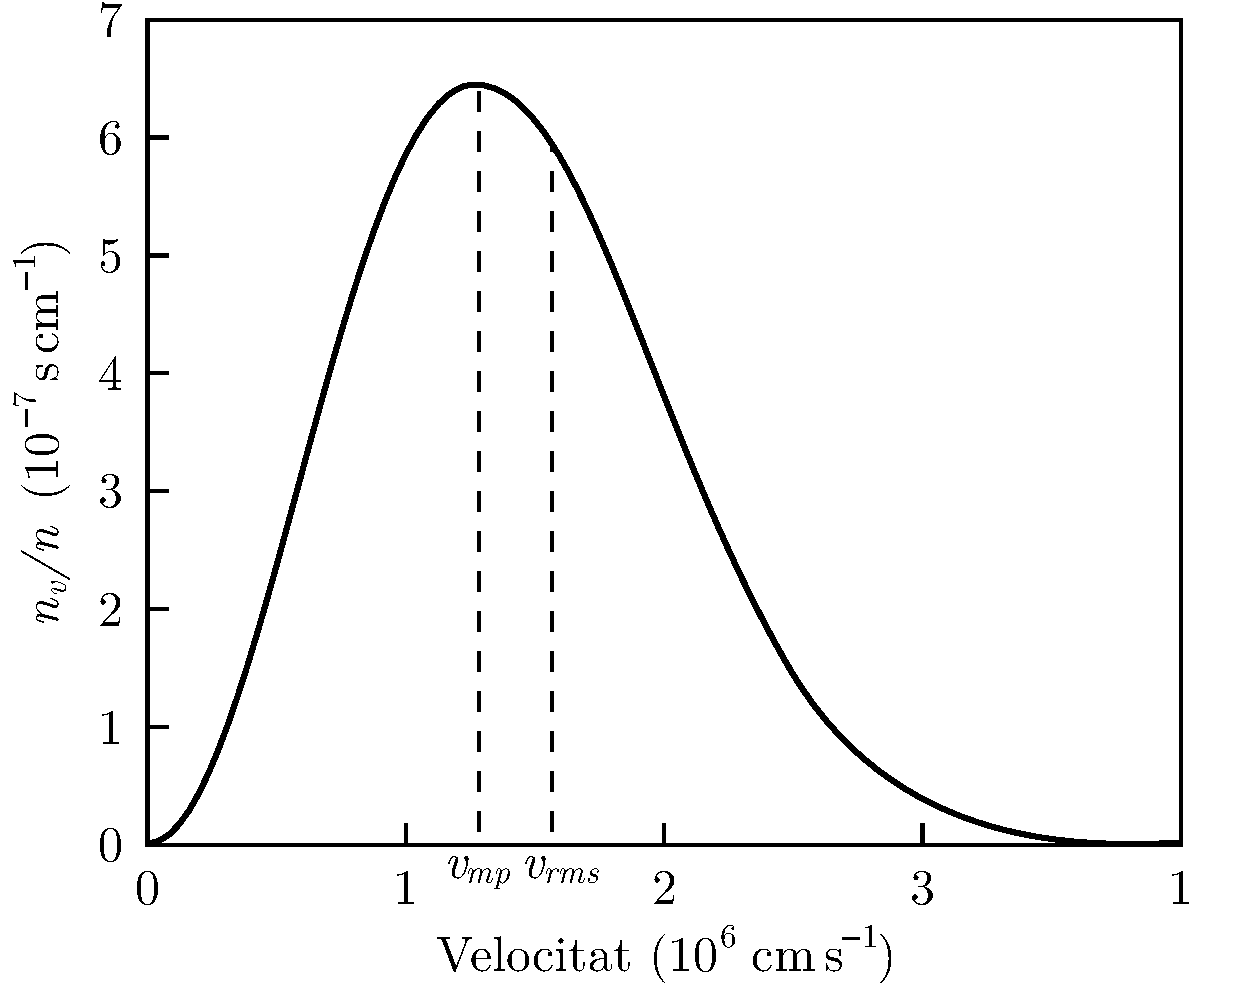
\includegraphics[width=0.65\textwidth]{./images/3-maxwell-boltzmann}
	\caption{Distribució de Maxwell--Boltzmann per a àtoms d'hidrogen a $T = \SI{10000}{\K}$, on $v_{mp} = \SI{1.29 e6}{\cm\per\s}$ i $v_{rms} = \SI{1.57 e6}{\cm\per\s}$}
	\label{fig:maxwell-boltzmann}
\end{figure}

La cua de la distribució cau aproximadament com $\exp[-\dfrac{mv^{2}}{2k_{B}T}]$.

La mecànica estadística ens diu que el quocient entre el nombre d'àtoms en dos estats idèntics $a$ i $b$ accessibles al sistema (el qual es troba en equilibri termodinàmic) és
\begin{align}
	\frac{N_{a}}{N_{b}} = \frac{g_{b}}{g_{a}} \exp[- \frac{E_{b} - E_{a}}{k_{B} T}]
\end{align}
on $g_{a}$ i $g_{b}$ són el nombre d'estats amb energies $E_{a}$ i $E_{b}$, respectivament, és a dir, la degeneració. Per a l'àtom d'hidrogen $g_{H,n} = 2n^{2}$.
\begin{example}
	Sigui un gas d'àtoms neutres d'hidrogen. A quina temperatura hi haurà igual nombre d'àtoms en l'estat fonamental que el primer estat excitat?
	\begin{align*}
		\frac{N(n=1)}{N(n=2)} = \frac{2\times 2^{2}}{2\times 1^{2}} \exp[\frac{13.6}{k_{B}T} \qty(\frac{1}{2^{2}} - \frac{1}{1^{2}})] \equiv 1 \Rightarrow T = \SI{8.54 e4}{\K}
	\end{align*}
\end{example}

Igualment, el nombre relatiu d'àtoms en diferents estats d'ionització ve determinat (en l'equilibri) per la temperatura segons l'equació de Saha~\eqref{eq:saha}.
\begin{figure}[h]
	\centering
	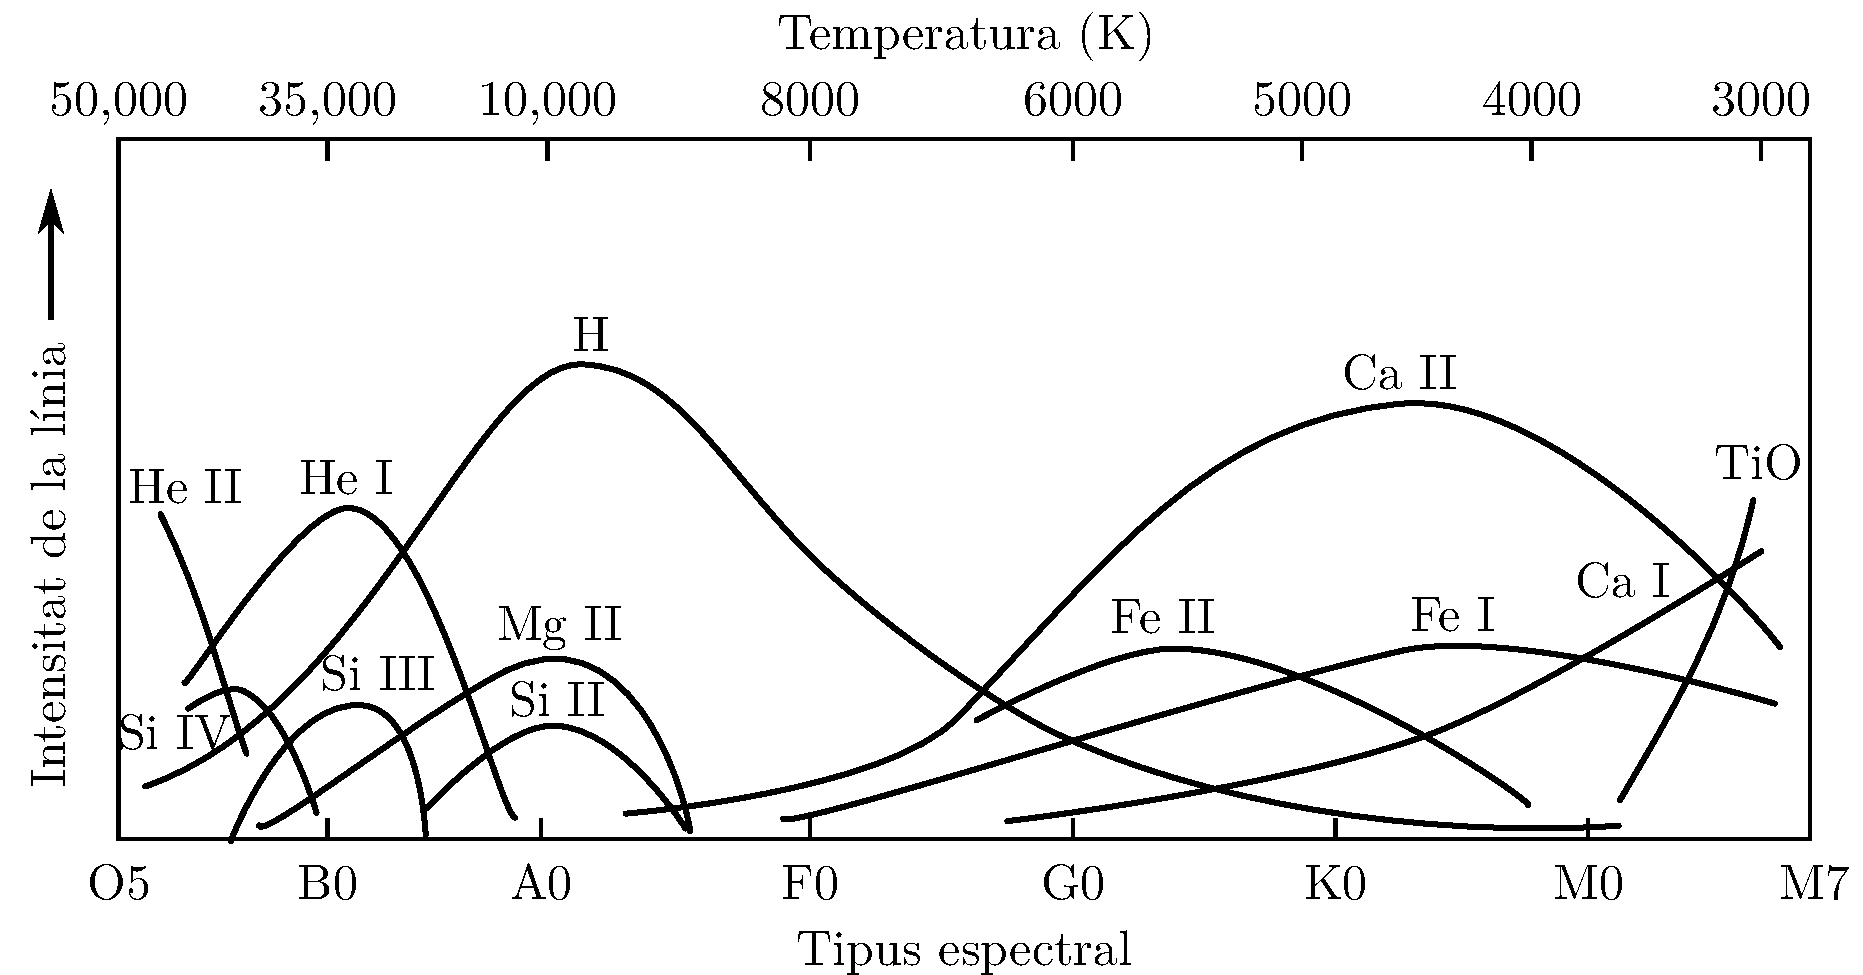
\includegraphics[width=0.95\textwidth]{./images/3-spectral-strenght}
	\caption{Dependència de les intensitats de les línies espectrals amb la temperatura}
	\label{fig:spectral-strenght}
\end{figure}

Per exemple, en l'equació de recombinació--ionització $e^{-} + p \leftrightarrows \ch{H} + \gamma$, la condició d'equilibri tèrmic és
\begin{align*}
	\mu(e^{-}) + \mu(p) = \mu(\ch{H}), \quad \qty[\mu(\gamma) \equiv 0]
\end{align*}
Aquesta condició condueix a
\begin{align}\label{eq:saha}
	\frac{x^{2}}{x-1} = \frac{1}{n} \qty[\frac{2\pi m_{e} k_{B} T}{h^{2}}] e^{-B/K_{B}T}
\end{align}
on $B = \SI{13.6}{\eV}$ és l'energia d'ionització, $x= n_{e}/n_{p}$, i $n = n_{p} + n_{H}$.
% \begin{sproof}
%     TODO: proof (class)
%     \url{https://en.wikipedia.org/wiki/Saha_ionization_equation}
% \end{sproof}

Llavors, el conjunt de línies espectrals d'una estrella ens proporciona informació no només de l'abundància relativa d'elements químics en les capes més externes, sinó també sobre el tipus espectral (O, B, A, etc.), estats d'ionització, i pressió (ja que a l'equació de Saha $n_{e}$ pot substituir-se per $p_{e} = n_{e} K_{B}T$).

%-----------------------------------------------------------------
\subsection{Efecte Doppler}
En general els espectres estel·lars es veuen desplaçats respecte els seus corresponents al laboratori. Això és degut a l'efecte Doppler.
\begin{figure}[h]
	\centering
	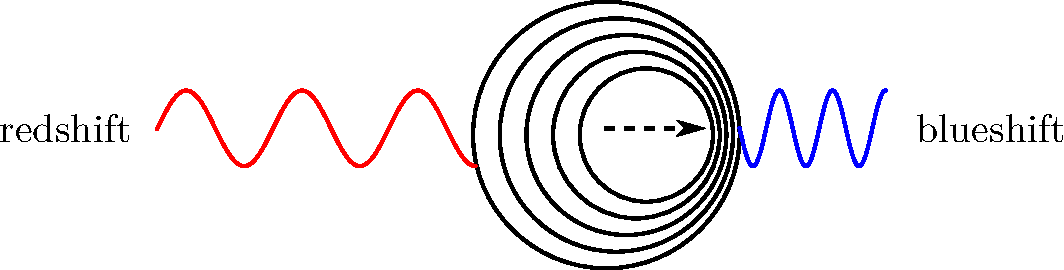
\includegraphics[width=0.7\textwidth]{./images/3-doppler}
	\caption{Quan la font de llum s'allunya de l'obsrvador, es produeix un \textit{redshift}, mentre que si la font s'hi apropa, es produeix un \textit{blueshift}}
	\label{fig:doppler}
\end{figure}

Si la velocitat radial (velocitat al llarg de la visual), $v_{r}$, de l'estrella és baixa ($v_{r} \ll c$), tenim
\begin{align}
	\frac{\Delta \lambda}{\lambda} = \frac{\lambda_{obs} - \lambda_{em}}{\lambda_{em}} = \frac{v_{r}}{c}
\end{align}
la qual cosa permet determinar $v_{r}$ amb una aproximació de $\SI{\pm10}{\m\per\s}$.

Per determinar $v_{\theta}$ (perpendicular a $v_{r}$) és necessari conèixer la distància a l'estrella, sigui aquesta $d$, i el seu desplaçament angular per unitat de temps, $\mu$, (típicament en $\si{\arcsecond\per\year}$), la qual cosa s'aconsegueix a través de l'observació durant un període de temps suficientment llarg. Es veu fàcilment que
\begin{align}
	v_{\theta} = \mu d
\end{align}

La velocitat de l'estrella respecte al Sol serà, doncs
\begin{align}
	v = \sqrt{v_{r}^{2} + v_{\theta}^{2}}
\end{align}
La velocitat mitjana del conjunt d'estrelles més pròximes al Sol és d'uns $\SI{25}{\km\per\s}$.

En realitat, la determinació de $v_{r}$ no és molt simple, ja que s'ha de tenir en compte la velocitat ($\approx$ constant) de la Terra en la seva òrbita solar ($\SI{29.8}{\km\per\s}$). Això dóna lloc a que $\lambda_{obs}$ variï sinusoïdalment al llarg de l'any. No obstant això, només cal restar (o sumar) la component de la velocitat terrestre al llarg de la visual per obtenir la vertadera velocitat radial de l'estrella respecte al Sol.

%-----------------------------------------------------------------
\subsection{Espectrògraf}
S'utilitza per determinar l'espectre d'estrelles i galàxies. Es fa passar la llum estel·ar per una escletxa, es col·lima mitjançant un mirall i es dirigeix sobre una xarxa de difracció. L'espectre resultant de la xarxa s'enfoca sobre una placa fotogràfica o sobre un detector electrònic.

La xarxa de difracció (una llarga sèries de doble escletxes molt pròximes entre elles) dóna lloc a màxims i mínims de difracció. Sigui $a$ la separació entre dues escletxes adjacents, llavors, es compleix
\begin{align}
	a \sin \theta = n \lambda, \quad n \in \mbb{N}
\end{align}
on $\theta$ és l'angle de difracció i $n$ és l'ordre de l'espectre.
\begin{figure}[H]
	\centering
	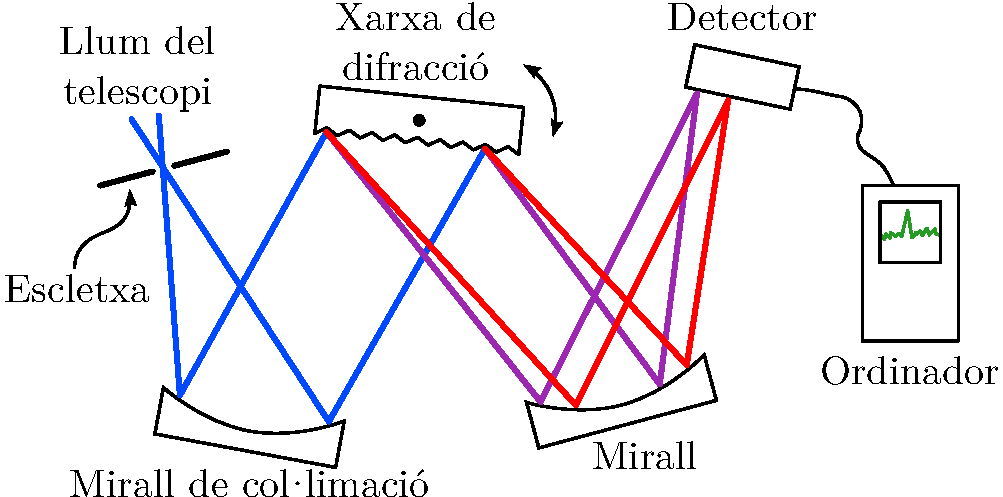
\includegraphics[width=0.65\textwidth]{./images/3-spectrograph}
	\caption{Diagrama d'un espectrògraf}
	\label{fig:spectrograph}
\end{figure}

La capacitat de resoldre dues longituds d'ona molt pròximes, separades per $\Delta \lambda$, depèn de l'ordre $n$ de l'espectre i del nombre total $N$ d'escletxes il·luminades.

La màxima resolució a la qual l'espectrògraf pot arribar és
\begin{align}
	\Delta \lambda = \frac{\lambda}{nN}
\end{align}
El quocient $\Delta \lambda / \lambda$ ens dóna el poder de resolució de la xarxa de difracció (a menor quocient, major poder).

%-----------------------------------------------------------------
\subsection{Diagrames de Hertzsprung--Russell}\label{sec:hertz-russell}
Si s'accepta que la superfície d'una estrella es comporta, aproximadament, com un cos negre, tindrem una relació entre la seva lluminositat $L$, el seu radi $R$, i la seva temperatura efectiva $T_{e}$:
\begin{align}\label{eq:hertz-russell}
	L = 4 \pi R^{2} \sigma T_{e}^{4}
\end{align}
on $\sigma$ és la constant d'Stefan--Boltzmann.

Aquesta relació és consistent amb el diagrama proposat per Hertzsprung (1905) i, independentment, per Russell (1912).

El radi d'una estrella pot calcular-se a partir de l'equació \eqref{eq:hertz-russell} i la seva posició al diagrama de Hertzsprung--Russell.

És important destacar les següents franges dels diagrames de Hertzsprung--Russell:
\begin{itemize}
	\item Una franja aproximadament diagonal (en què es troba el Sol) amb $\SI{0.1}{\Rsun} \leq R \leq \SI{20}{\Rsun}$. Aquesta franja s'anomena \textit{seqüència principal}.
	\item Una franja d'estrelles gegants (a dalt de la zona inferior de la seqüència principal) amb $\SI{10}{\Rsun} \leq R \leq \SI{100}{\Rsun}$.
	\item Una altra franja, menys poblada, de supergegants amb radis $\sim \SI{e3}{\Rsun}$.
\end{itemize}
\begin{figure}[h]
	\centering
	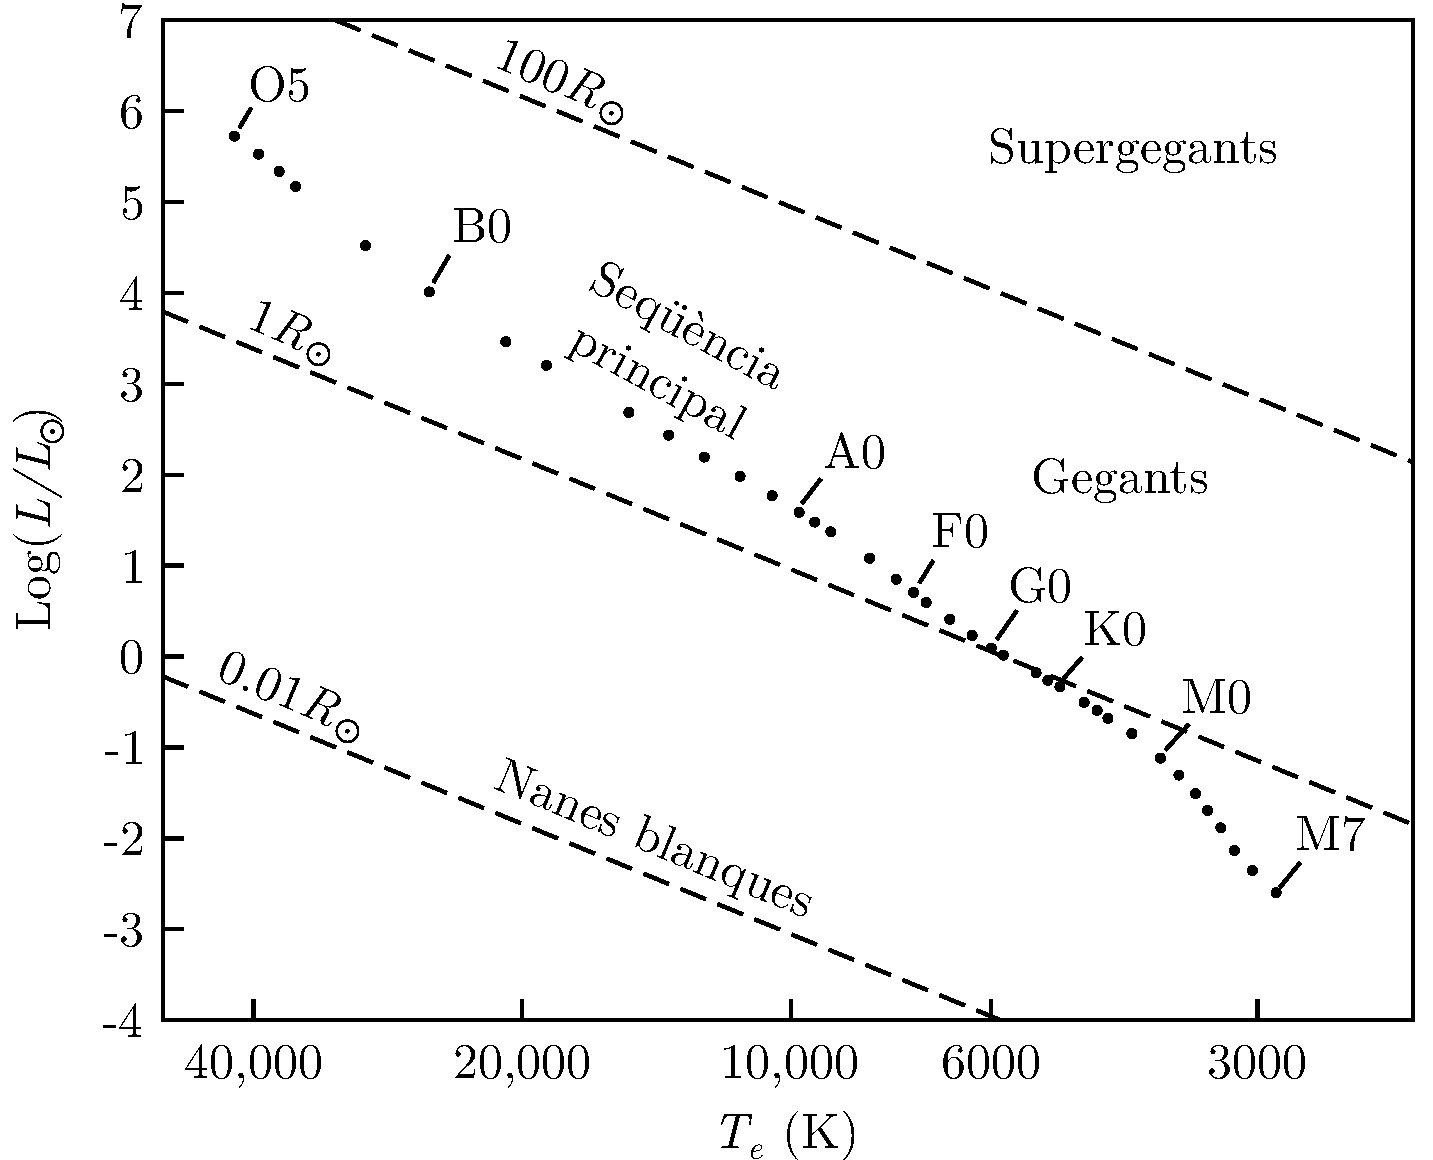
\includegraphics[width=0.75\textwidth]{./images/3-hertzsprung-russell}
	\caption{Diagrama de Hertzsprung--Russell teòric. Les línies discontínues indiquen les estrelles de radi constant.}
	\label{fig:hertzsprung-russell}
\end{figure}

El rang de lluminositats estel·lars és aproximadament de
\begin{align*}
	\SI{5 e-4}{\Lsun} \lesssim L \lesssim \SI{e6}{\Lsun}
\end{align*}
Sobre la seqüència principal es dóna la relació lluminositat--massa
\begin{align}
	\frac{L}{\Lsun} \propto \qty(\frac{M}{\Msun})^{\nu}, \quad \text{on } \nu = \begin{cases} 1 & \text{estrelles molt massives} \\ 3 & \text{estrelles massives} \\ 5.5 & \text{estrelles poc massives} \end{cases}
\end{align}
La densitat en les estrelles de la seqüència principal és $\sim \SI{1}{\g\per\cubic\cm}$.
\begin{itemize}
	\item El Sol és una estrella de la seqüència principal de tipus espectral G2. $\Msun = \SI{1.988 e 33}{\g}$, $\Rsun = \SI{6.955 e10}{\cm} \Rightarrow \rho_{\odot} = \SI{1.411}{\g\per\cubic\cm}$.
	\item Sírius, l'estrella més brillant del firmament nocturn, és del tipus espectral A1. $M_{S} = \SI{2.3}{\Msun}$, $R_{S} = \SI{1.6}{\Rsun} \Rightarrow \rho_{S} = \SI{0.792}{\g\per\cubic\cm}$.
\end{itemize}
En canvi, les gegants i supergegants són molt menys denses.
\begin{itemize}
	\item Betelgeuse ($M_{B} \approx \SI{12}{\Msun}$) és una estrella polsant de radi màxim de $\SI{e3}{\Rsun}$. Llavors, té una densitat de $\rho_{B} \sim \SI{e-8}{\g\per\cubic\cm}$, menys densa, doncs, que l'aire a nivell del mar.
\end{itemize}

\begin{example}
	La temperatura efectiva d'una estrella és $T_{e} = \SI{12000}{\K}$ i la seva magnitud absoluta és $M = 0.0$. Trobeu el seu radi sabent que la temperatura efectiva del Sol és $T_{e,\odot} = \SI{5800}{\K}$ i la seva magnitud absoluta és $\Msun = 4.76$.

	Recordem que si dues estrelles es troben a la mateixa distància de la Terra, la relació entre les seves magnituds absolutes és $M_{1} - M_{2} = - 2.5 \log (L_{1}/L_{2})$, i si una de les estrelles és el Sol, llavors
	\begin{align*}
		M - \Msun = - 2.5 \log(\frac{L}{\Lsun})
	\end{align*}
	Tenint en compte que $L = 4 \pi R^{2} \sigma T_{e}^{4}$, s'arriba a
	\begin{align*}
		M - \Msun = - 2.5 \qty[ 2\log(\frac{R}{\Rsun}) + 4\log( \frac{T_{e}}{T_{e,\odot}} ) ]
	\end{align*}
	és a dir
	\begin{align*}
	\begin{aligned}
		-\qty(\frac{M-\Msun}{5}) &= \log \qty[\qty(\frac{R}{\Rsun}) \qty(\frac{T_{e}}{T_{e,\odot}})^{2}]\\
		\Rightarrow \frac{R}{\Rsun} &= \qty(\frac{T_{e,\odot}}{T_{e}})^{2} 10^{-(M-\Msun)/5} \approx 2
	\end{aligned}
	\end{align*}
	Llavors $R \approx \SI{2}{\Rsun} = \SI{1.391 e6}{\km}$.
\end{example}
